%! TEX root = diss.tex
\documentclass[../diss.tex]{subfiles}
\chapter{Implementation}

% NOTE: Multiprocessor => shared memory. Use term "parallel computer" instead

% Introduction:
% * TODO: change fig 2.1 to have cloud of "graph data.csv" that interact with
%   "input graph"
% * Refer to figure 2.1, go into some more depth on interface to Parallel
%   system simulation:
%   * You create Worker implementation with access to ...., then pass
%     description to manager, specify number of workers, topology to use, num
%     computation phases, etc.
% * _Intrdc the different components, and then start going into detail in ind. subsecs_

% Some "practices used/software dev.? chapter":
% * Weekly meetings, log book,

% Graph datasets:
% * California road networks:
%   * freely-available, consisten format, real-life road network
% * Random graphs:
%   * To satisyf req. of different n
%   * Erdos-Renyi graph, but modified to be fully-connected, trick to get same properties
%     with formula for creating $p$
%   *  python library used
% * Graph reader
%   * adjacency matrix and also neighbourhood list for Dijkstra's algorithm
% * TODO: mention networkx as well as GraphReader class
% Graph datasets {{{
\section{Graph datasets}%
\label{sec:Graph datasets}

To run the algorithms, we need graphs as input. Since one important usage of \ac{APSP}
is route-planning, I used a dataset of the Californian road-network. This dataset was
initially used in \citep{graph-dataset} and has been made available on the author's
website\footnote{\url{https://www.cs.utah.edu/~lifeifei/SpatialDataset.htm}}.
% TODO: add plot of the dataset as a figure, using the python script...
This graph was used to prove that practical problems can quickly be solved on my
simulated parallel system, as long as graph compression is used.
However, for evaluation I needed graphs of various sizes, so these were generated
randomly.

\subsection{Random graph generation}%
\label{sub:Random graph generation}

% TODO: information on Erdos-Renyi graphs in prepreration chapter...

I chose to use Erd{\"o}s-Renyi graphs because they have previously been used in
evaluation of \ac{APSP} algorithms.
% TODO: cite https://core.ac.uk/download/pdf/81103122.pdf
%            https://www.researchgate.net/publication/47842024_A_Parallelization_of_Dijkstra%27s_Shortest_Path_Algorithm
I have tried to fit the parameters as closely to the real-world graph datasets
as possible. There are many characteristics of a graph, such as vertex- and
edge-connectivity, betweenness centrality, clustering coefficient, and average
distances. However, trying to generate new graphs with similar values for all
of these metrics quickly becomes a difficult problem. I have therefore only
tried to replicate the metric, \textit{average vertex degree}, which should
have some correlation to the mentioned metrics. I also want the random graphs
to be fully-connected, as most road-networks are. In the $G(n,p)$ random-graph
model, the graph is constructed by starting with a set of $n$ vertices, and
then independently include every possible edge $e$ with
% (TODO: citation???)
probability $p$. This makes the edges follow the binomial distribution:
\begin{equation}
    \textrm{deg}(v) \sim \textrm{Binomial}(n-1,p)
\end{equation}
with the average degree being $(n-1)p$. However, by instead starting with a
\textit{circular graph} and including each remaining edge independently with
probability
\begin{equation}
    p=\frac{\textrm{desired average degree} - 2}{n - 3},
\end{equation}
we get a fully-connected graph where the average degree is as desired.
% TODO: proof in appendix...
I chose the desired average degree based on the Californian road-network, which
is 2.061. However, since we will be using the compressed graph (see
\autoref{sec:Graph compression}), I used the average vertex degree of the
compressed California graph instead, which was 2.945. In
\autoref{fig:example-graph-random}, I have plotted an example graph generated
through this method. I then generated ? graphs of various sizes, from 10 nodes
to 700 nodes for use in evaluation. %TODO: how many?

\begin{table}
    \centering
    \begin{tabular}{|c|c|}
        \hline
        \textbf{Location} & \textbf{Average vertex degree} \\
        \hline
        San-Francisco (SF) &  2.549 \\
        \hline
        North-America (NA) & 2.038 \\
        \hline
        ? (OL) & 2.305 \\
        \hline
        California (cal) & 2.061 \\
        \hline
        ? (TG) & 2.614 \\
        \hline
    \end{tabular}%
    \caption[Caption]{Average vertex degree for various road-network datasets\footnotemark.}%
    \label{tab:vertex-degree}
\end{table}

\footnotetext{These values were computed using the TODO??? method in \texttt{GraphReader}.}

\begin{figure}
\begin{center}
    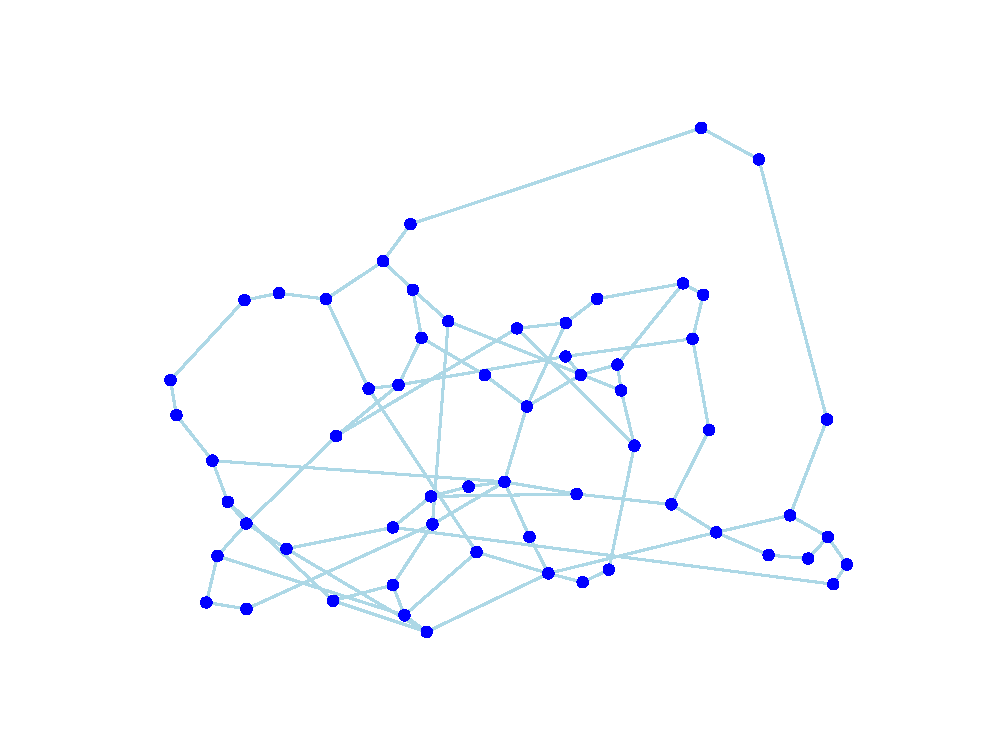
\includegraphics[scale=.7]{figs/plots/example-graph.eps}
\end{center}
\caption[Caption]{A visualisation of a graph generated with the modified
Erd{\"o}s-Renyi model. The graph has $n=60$ vertices, and the length of the
edges correspond to their weight\footnotemark[3].}%
\label{fig:example-graph-random}%
\end{figure}

\footnotetext[3]{The graph was visualised using the \texttt{ForceAtlas2} library in python. See TODO}

% \begin{algorithm}
%     \caption{Fully-connected random graph with specific average degree}%
%     \label{alg:random-graph}
%     \KwData{$n$, avg\_degree}
%     \KwResult{$G=(V,E)$}
%
%     $G \leftarrow (\textrm{set of } n \textrm{ vertices}, \emptyset)$
%
%     \For{vertices $v_{i}, v_{i+1}$}{
%         $E \leftarrow E \cup (v_{i}, v_{i+1}, w), \textrm{ where } w \sim \textrm{Uniform}[0,1]$
%     }
%     $E \leftarrow E \cup (v_{0}, v_{n-1}, w), \textrm{ where } w \sim \textrm{Uniform}[0,1]$
%
%     Not finished....
%
% \end{algorithm}


% }}}

% Simulation of a distributed memory multiprocessor:
% * Introduction:
% *   Overview of the components in bigger UML diagram, and comments on their interaction
% * Memory model (?)
%   * explain design decision behind Map : (label : String) -> (value : Number)
%   * ...
% * Timing analysis
%   * implemented as decorators for the system simulation
%   * Explain equations for how MIMD simulated (stalling bc. wait, latency+bandwidth etc.
%   * Repating computation measures, cache misses effect, possible bc.
%     seperation, mask read writes to ensure same computation done,
%     goal is more accurate eval
% Simulation of a distributed memory multiprocessor {{{
\section{Simulation of a distributed memory multiprocessor}%
\label{sec:Simulation of a distributed memory multiprocessor}

% TODO: Introduction, here we want to present the reader with the four phases and
%  the **interface** we want to create, as if reader sees diagram first, will
%  have no idea _what_ the communicationBefore, etc. is and why it's there
% * The parallel algorithms, including possible extensions, can be split into
%   3/4 phases
% * Doing this also has many benefits (TODO: go through diary and find
%   the benefits)
% * The diagram with parallel communicationBefore, then memory flush, sync barrier,
%   followed by another repeated execution, that diagram goes here and is
%   refered to

% In this "introduction 2" chapter, we explain the diagram...
\subsection{Overview of components}%
\label{sub:Overview of components}

% TODO: add comment that Manager runs whatever methods on the worker objects it has
% TODO: also add number annotations, showing how many of each they have
% TODO: shorten width of ComMan, so that can have some blue on the side
\begin{figure}[h]
\begin{center}
    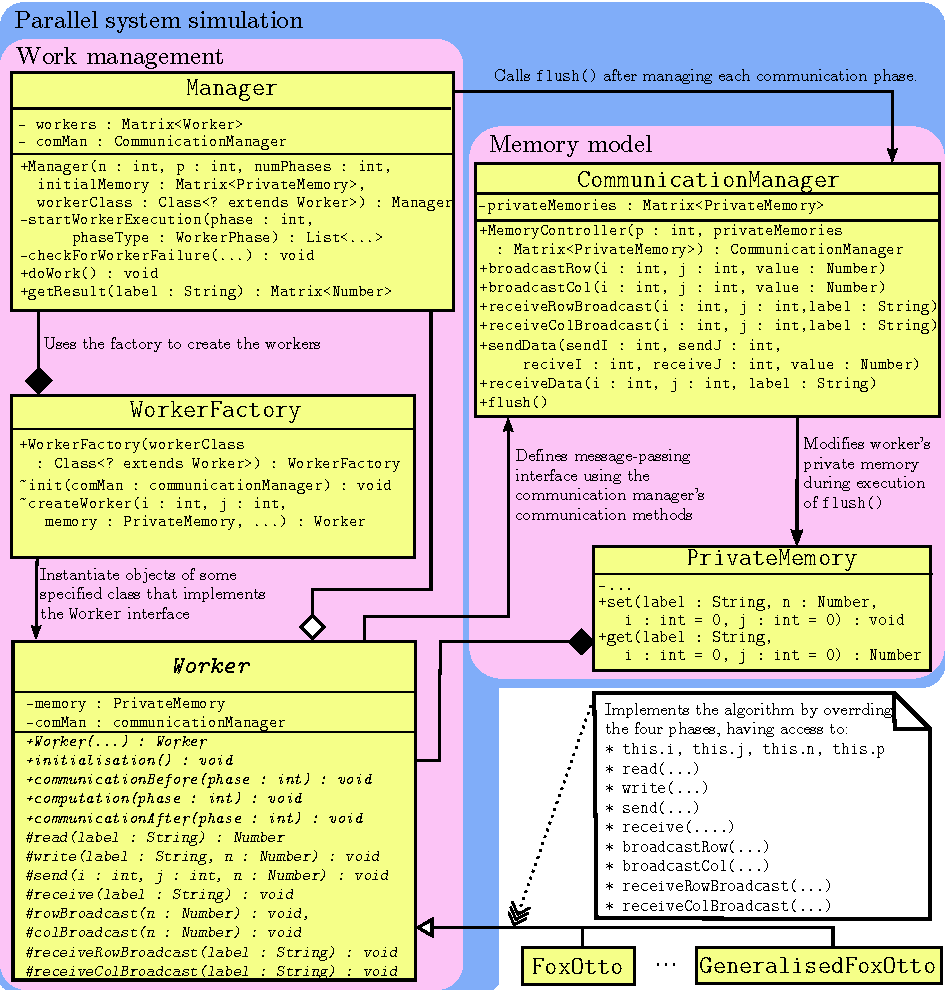
\includegraphics[scale=1]{figs/parallel-system-simulation.pdf}
\end{center}
\caption{A overview of the classes and their interaction in simulator.}
\label{fig:parallel-system-overview}
\end{figure}

In \autoref{fig:parallel-system-overview}, we see an overview of the main
components of the simulator, and how they interact. The \texttt{Manager}
constructs the specified number of \texttt{Worker}s based on some provided
subtype e.g.~\texttt{FoxOtto}, using a \texttt{WorkerFactory}. When
\texttt{doWork()} is called, it will then run the \texttt{Worker}s through all
of their communication- and computation-phases, and \texttt{flush()} the
effects of their communication after each phase, which is done using the
\texttt{CommunicationManager}. The \texttt{Worker} is an abstract class
and provides a simple yet expressive interface for algorithms ....

% Work management points:
% * Diagram of how work is simulated in parallel fashion, 8 blocks at a time
% * Use Java's executor service to avoid thread management overhead
% * Briefly remind about interace, and communication method using one object
% * Manager explain, from construction, to how doWork works, to getResult, also
%   allowing reuse of workers, which is nice ...
% * Worker factory
%   * Use of reflection, so can allow arbitrary description to be passed and
%     can still
%     crete the new worker objects that can be managed
\subsection{Work management}%
\label{sub:Work management}

When constructing the \texttt{Manager}, we specify the number of \acp{PE},
their initial memory content, and what computation they should do in each phase,
which is done by specifying the class of some implementation of
\texttt{\textit{Worker}}. When calling \texttt{doWork()} on the manager, it will
then run all the workers through a specified number of phases, where there is
3 subphases in each phase. Looking at a single worker in isolation, the execution
can be seen in \autoref{alg:execution-order}. However, these tasks are simulated
in parallel, and we must run the same subphase of all the workers before moving
onto the next because of data dependencies. This parallel execution order is
visualised in \autoref{fig:work-management-blocks}. After this is done, we can
call \texttt{getResult(label)} to extract the result by combing the
private memory of each worker into a matrix.

The worker done by each \ac{PE} is specified in subphases.  When investigating
the different algorithms, as well as possible extension like Floyd-Warshall, I
realised that they all had clear distinctions between when the \acp{PE} were
doing computation and when they were communicating. This made forcing such a
distinction in the interface not induce a reduction in flexibility. Instead of
providing an abstract method \texttt{work}, where the programmer would themself
create a \texttt{for}-loop and combine communication and computation, we
provide the four methods shown in \autoref{fig:parallel-system-overview} and
execute them as shown in \autoref{alg:execution-order}.

% TODO: can the above two paragraphs be combined somehow?

\begin{wrapfigure}{l}{0.5\textwidth}
\begin{minipage}{0.5\textwidth}
    \begin{algorithm}[H]
    \caption{Execution of phases of some worker id $(i,j)$}%
    \label{alg:execution-order}

worker.initialisation();

\SetKwComment{Comment}{/* }{ */}
\For{$l = 0 \dots \textrm{number of phases} -1$}{
    \texttt{worker.communicationBefore($l$)}

    \texttt{worker.computation($l$)}

    \texttt{worker.communicationAfter($l$)}

}
\end{algorithm}
\end{minipage}
\end{wrapfigure}

Splitting up the work phases allows them to be represented as independent
\texttt{Callable} tasks, which has many benefits. Firstly, it allows managing
the workers using higher-level constructs like a Java \texttt{ExecutorService}
rather than using Java \texttt{Thread}. We can submit all the $p^2$ tasks in a
subphase to the executor service, and it will complete all of them without ever
spawning more than 16\footnote{This number is configurable, but since my Laptop
can execute 16 threads simultaneously, this was the optimal number} threads,
which avoids a lot of overhead. Additionally, as I will explain further in the
memory model, the side-effects of communication only happen when
\texttt{CommunicationManager::flush} is called, so there are no data
dependencies between \acp{PE} within a subphase, only between two different
subphases. Therefore I do not need locking mechanisms inside the
\texttt{\textit{Worker}}, but can instead implicitly implement them by
executing them in the order shown in \autoref{fig:work-management-blocks}.  The
third benefit is allowing repeated execution of the same work, which gives a
more accurate timing estimate.
% TODO: mention additional benefit: Easy to handle exceptions thrown by workers
%       and report them back to the caller while cleanly stopping all threads,
%       which makes development of the algortihms a lot easier, because can e.g.
%       see if receive's and send's are mismatched

% TODO: alternative diagram:
%   very small blocks with different colours, and the colours indicate whether it's
%   initilisatin, comBefore, compu, etc., and text inside is just e.g. "(0,0)"...
\begin{figure}
\begin{center}
    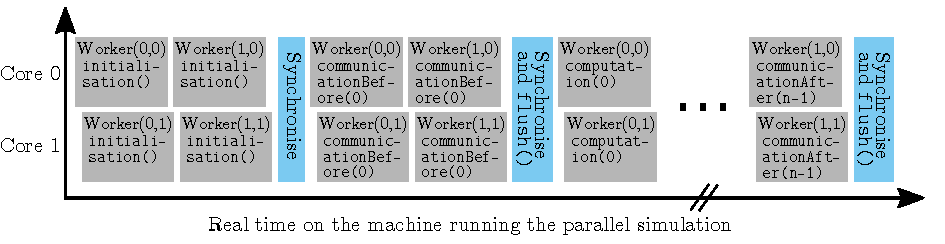
\includegraphics[scale=1]{figs/work-management-blocks.pdf}
\end{center}
\caption{Example of multithreading when simulating a 4 processing elements on
a host computer with 2 cores.}
\label{fig:work-management-blocks}
\end{figure}

The \texttt{WorkerFactory} uses Java's reflection API to create instances of
any implementation of the \texttt{\textit{Worker}} interface. When constructing
this factory, by provide a \texttt{Class} object of for instance the
\texttt{FoxOtto} implementation. It can then infer the appropriate constructor
at runtime and create $p^2$ \texttt{FoxOtto}-workers, without there being need
for a dedicated Fox-Otto worker factory. This simplifies the parallel programming
interface as implementing \texttt{\textit{Worker}} is all that is needed to
add an additional parallel algorithm to the system.

\subsection{Memory model}%
\label{sub:Memory model}

% Explains string label access
Memory is accessed through string labels. The communication
Each \ac{PE} has its own local memory, represented by a \texttt{PrivateMemory}
object. To make access as easy to use as possible for the programmer, access
is done through string labels. For example, a \ac{PE} can store some values
at location \texttt{"A"} and then retrieve it with the same label later,
additionally, for \acp{PE} handling a non $1\times 1$-sub-matrix, the
local memory is arranged in a matrix where the \ac{PE} can for instance store
values at location \texttt{(1,4,"A")} to associate it with some result related
to for example $C_{5,9}$.
% TODO: explain better above

% Communication
Introduction. To send for example data with point-to-point connections, both
the sender and recipient must call \texttt{sendData} and \texttt{receiveData},
respectively. The \texttt{receiveData(i, j, label)} method does not return a
value, but instead causes the recipient's memory at label \texttt{label} to be
set to whatever value was received. This change does not happen until
\texttt{CommunicationManager::flush()} is called, which happens in the
synchronisation phase in ?.% TODO: reference
During the flushing all the sent data is matched up with corresponding calls
to \texttt{receiveData}, and the private memories of all the recipient is
modified by the \texttt{CommunicationManager}.
An obvious alternative to this approach is making the \texttt{receiveData} method
return the actual number received, which can be done by putting the recipient
Thread to sleep until another thread has sent it data. My approach has the
following benefits and drawbacks:
\begin{itemize}
    \item[+] Separating the computation and communication gives implicit thread
        synchronisation, which allows using fewer \texttt{Thread}s, causing
        less overhead (see ) % TODO: reference manager
    \item[+] Measuring the computation time for evaluation is a lot simpler
    \item[$-$] Computation must be interleaved with a communication phase and
        we get less flexibility for algorithms where these two phases cannot
        be cleanly seperated
    \item[$-$] The \texttt{receiveData} method not returning anything is not
        an intuitive abstractions, but rather requires the programmer to know
        slightly more about the implementation of the \texttt{CommunicationManager}
\end{itemize}
% TODO: write something about how ties ties in with seperating the phases?

The main benefits are making the work management simpler, and setting up for
more accurate evaluation. The first drawback is not relevant for the algorithms
I have used. % TODO: ?

\subsection{Estimating computation and communication times}%
\label{sub:Estimating computation and communication times}

% TODO: don't know what to name a ssub here...

% The points to introduce this sub section with are:
* Diagram of how communication causes stalls, counted as comTime:
  * Split up phases into the 3 things, and can use arrow to indicate which PE
    is sending to what, and assumption on if send-before, no delay to start
    next phase...
* What is measured as computation time
* The equation for estimating communication, latency + bandwitdh * w, and
  the assumptions made behind this

\subsubsection{The \texttt{timingAnalysis} package}

The functionality for measuring the computation time of each \ac{PE} and
estimating the communication time required for message-passing is implemented
using the \textit{decorator} pattern. In \autoref{fig:timing-analysis-overview},
we see an overview of the components of the \texttt{timingAnalysis} package,
where the green classes are implemented using decoration: They extend the
base class and only override methods related to timing, and use a reference to
the base object to perform the original functionality in addition to the added
timing analysis.

% TODO: blue background for what is part of the package....
\begin{figure}
\begin{center}
    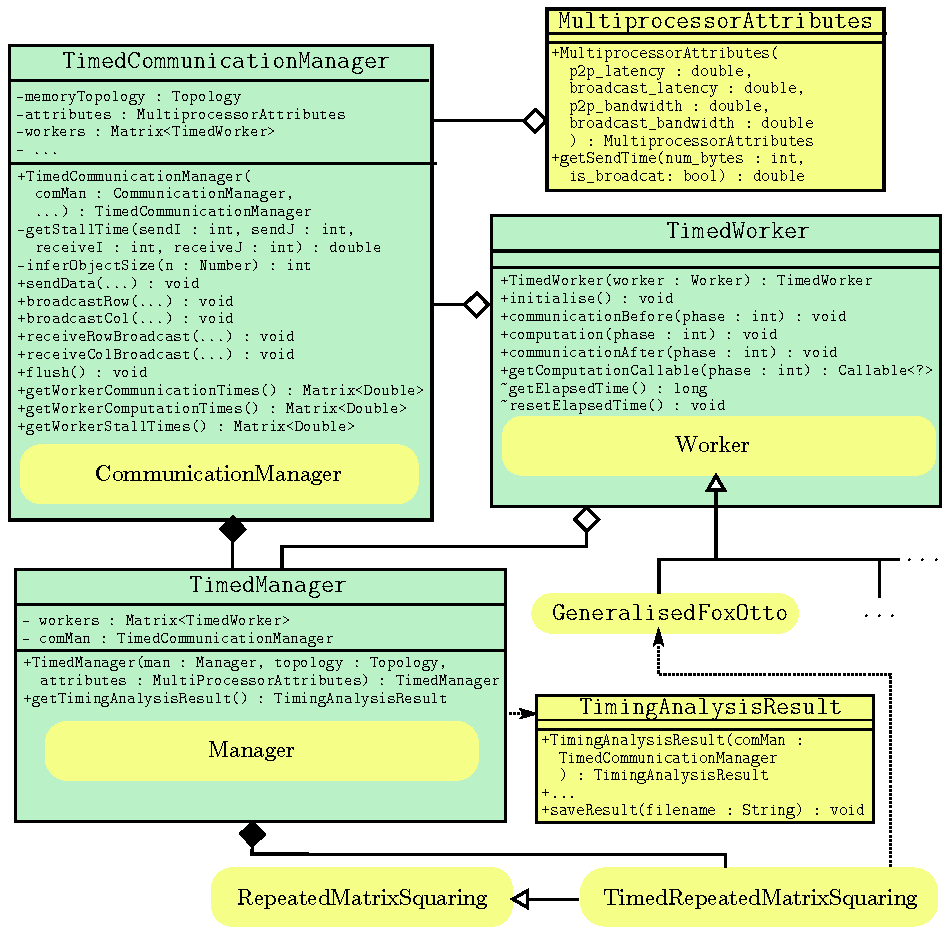
\includegraphics[scale=1]{figs/timing-analysis-overview.pdf}
\end{center}
\caption{A overview of the components of the \texttt{timingAnalysis} package.
Note that the \texttt{GeneralisedFoxOtto} and the \texttt{RepeatedMatrixSquaring}
classes are not part of this package. Additionally, the green class diagrams with
a yellow class inside it are short-hands for the decorator-pattern, where the
outer class extends the yellow inner one and contains a reference to it.}
\label{fig:timing-analysis-overview}
\end{figure}

% TODO: work from here, and write first paragraph with stuff, then about
%  TimedManager and TimedWorker in one par, then move onto below the advantages..
To explain:
* In multiprocessorAttributes, can specify constants to use (ref equations)
* These are used when computing message passing time in TimedComMan
* In that class, maintain a matrix of the simulated real-time of all the \acp{PE}
    and at each \texttt{flush()}, we update these based on stalling required
    by the senders (as explained above...)
* when the send or broadcast methods are called, we keep count of the number of
  bytes sent, reset on flush, combine all in same packet possible, so programmer
  don't need to worry about this. After this, do original functionality by
  using held reference
* In TimedManager, we decorate all the workers by constructing TimedWorker on them,
  and we replace the Manager's existing \texttt{Matrix<Worker>} with these
  using dynamic dispatch. TM also decorates the ComMan from the original Manager
* In the TimedWorker, we use Java's \texttt{ThreadMXBean} to find the CPU time
  each Worker spend on the CPU while running their \texttt{computation(phase :
  int)} We also use a clever trick to minimize other effects, repeat computation
  and take their average, not in cache, disable writes during this, so always
  same branch, etc.

Points to write in some last paragraph on why this good idea:
* By seperating the timing functionality, we make implementation easier and
  modularise further. When timing the program complete seperate task, so first
  focus on simulating processor, then focus on how to time this simulation. The
  distinction between SIMD and MIMD will also just be present here, so could
  for instance extend further with new decorator for SIMD
* Also follow principle of each class doing one thing, so additional functionality
  for e.g. repeated execution not mixed with the standard worker behaivour
* The interaction between the components above are not all explicitly redone in
  the decorators, but are instead present from the components underneath. For
  instance manager, just decorates all the workers the manager already have
  created with the WorkerFactory
* How MIMD works, the stalling time etc., explained with a diagram...

Components:
* MultiprocessorAttributes
* TimedManager
* TimedRepeatedMatrixSquaring
* TimedWorker
* TimingAnalysisCommunicationManager
* TimingAnalysisResult

% }}}

% APSP via repeated matrix-squaring
% * Can abbriviate as MatSquare or something
% * Start with top-down explanation, what happens when do A^2 and same for pred. matrix
% * Then explain the driver code, why this number of iterations etc.
% * Then explain generalized fox otto algorithm, noting special case for pred. matrix
% * Explain FoxOtto (explain predecessor functionality and edge-case,
%   generalized version, pseudo-code, diagram of memory movement can go in preparation)
% * Explain driver code, and its complexity?
% * As explain, also use a simple graph as an example, going through as you do the
%   general explanation
% APSP via repeated matrix-squaring {{{
\section{APSP via repeated matrix-squaring}%
\label{sec:APSP via repeated matrix-squaring}

The \emph{\acl{MatSquare}} algorithm, which I will abbreviate as \emph{\acs{MatSquare}},
is an algorithm. \acused{MatSquare}
By using \ac{MatSquare}, we can ...


% Notes from reserach-and-planning diary:
% **Problem with generalized FoxOtto**:
% In the general version, we first started the multiplication by iterating from
% the top of the submatrix (see diagram in notes for $C_{10,6}$ for instance).
% However, this causes problems for the predecessor values because of the initial
% conditions. Consider the scenario for $C_{10,6}$ where want to compute path 10
% -> 10. Whenever we get to $k=10$, we would not assign predecessor because of
% exemption condition (which is necessary, otherwise we get other bugs). And at
% this point ($k=10$) we discover path of length 0. However, because of the
% generalization, we start with $k=8$ (ref. to diagram), so we find another path
% of longer length, and when we get to $k=10$, we optimize the path, but leave
% the predecessor as it was for the longer path because of the exemption
% condition. One fix is to save the initial "dist" and not use $\infty$ every
% time. Another option is making sure we start with $k=10$ when running algo i.e.
% being consistent with non-general version. That way, we immediately relax
% distance to 0 and keep the initial predecessor, this.j (or read("P") which is
% same thing). This is the option I went for, and is the reasoning behind the `m`
% loop and then modifying `iter`.
%
% * In `CountingMemoryController`, we assume
% that each PE only sends data to **one** other PE, but this is NOT CHECKED
% anywhere. However, it is enforced in underlying memory controller that each PE
% can only receive from **one** other PE, which is not equivilant, but in _most
% cases_ (all PE do the same thing) causes the above assumption to hold.

% }}}

% Graph compression:
% * The algorithm for this, and explain all the edge cases, **with diagrams**
% * Also simple graph to use as an example
% * Also a section for the expected asymptotic speed-up referencing random graph generation
% Graph compression {{{
\section{Graph compression}%
\label{sec:Graph compression}

% }}}

% vim: foldmethod=marker
